\begin{comment}
\documentclass[10pt]{article}
\usepackage{fullpage, graphicx, url}
\setlength{\parskip}{1ex}
\setlength{\parindent}{0ex}
\title{GEN12}
\begin{document}


\begin{tabular}{ccc}
The Alternative Csound Reference Manual & & \\
Previous & &Next

\end{tabular}

%\hline 
\end{comment}
\section{GEN12}
GEN12�--� Generates the log of a modified Bessel function of the second kind. \subsection*{Description}


  This generates the log of a modified Bessel function of the second kind, order 0, suitable for use in amplitude-modulated FM. 
\subsection*{Syntax}


 \textbf{f}
 \# time size 12 xint
\subsection*{Initialization}


 \emph{size }
 -- number of points in the table. Must be a power of 2 or a power-of-2 plus 1 (see \emph{f statement}
). The normal value is power-of-2 plus 1. 


 \emph{xint}
 -- specifies the \emph{x}
 interval [0 to \emph{+xint}
] over which the function is defined. 


 


\begin{tabular}{cc}
\textbf{Note}
 \\
� &

 


 
\begin{itemize}
\item 

  This subroutine draws the natural log of a modified Bessel function of the second kind, order 0 (commonly written as \emph{I}
 subscript 0), over the x-interval requested. The call should have rescaling inhibited. 

\item 

  The function is useful as an amplitude scaling factor in cycle-synchronous amplitude-modulated FM. (See Palamin \& Palamin, \emph{J. Audio Eng. Soc., 36/9}
, Sept. 1988, pp.671-684.) The algorithm is interesting because it permits the normally symmetric FM spectrum to be made asymmetric around a frequency other than the carrier, and is thereby useful for formant positioning. By using a table lookup index of \emph{I}
(r - 1/r), where \emph{I}
 is the FM modulation index and \emph{r}
 is an exponential parameter affecting partial strengths, the Palamin algorithm becomes relatively efficient, requiring only oscil's, table lookups, and a single \emph{exp}
 call. 


\end{itemize}


\end{tabular}

\subsection*{Examples}


  Here is a simple example of the GEN12 routine. It uses the files \emph{gen12.orc}
 and \emph{gen12.sco}
. It generates the function \emph{ln(I0(x))}
 from 0 to 20. Here is its diagram: 


 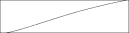
\includegraphics[scale=1]{gen12} 


 Diagram of the waveform generated by GEN12.


 \textbf{Example 1. A simple example of the GEN12 routine.}

\begin{lstlisting}
/* gen12.orc */
; Initialize the global variables.
sr = 44100
kr = 4410
ksmps = 10
nchnls = 1

; Instrument #1.
instr 1
  ; Create an index over the length of our entire note.
  kcps init 1/p3
  kndx phasor kcps

  ; Read Table #1 with our index.
  ifn = 1
  ixmode = 1
  kamp tablei kndx, ifn, ixmode

  ; Create a sine wave, use the Table #1 values to control
  ; the amplitude. This creates a sound with a long attack.
  a1 oscil kamp*30000, 440, 2
  out a1
endin
/* gen12.orc */
        
\end{lstlisting}
\begin{lstlisting}
/* gen12.sco */
; Table #1: a modified Bessel function (using GEN12).
f 1 0 2049 12 20
; Table #2, a sine wave.
f 2 0 16384 10 1

; Play Instrument #1 for 2 seconds.
i 1 0 2
e
/* gen12.sco */
        
\end{lstlisting}
\subsection*{Credits}


 Example written by Kevin Conder
%\hline 


\begin{comment}
\begin{tabular}{lcr}
Previous &Home &Next \\
GEN11 &Up &GEN13

\end{tabular}


\end{document}
\end{comment}
